% 5. Methodology I
\begin{frame}{Methodology I: Allometry \& Spatial Invariants}
    \begin{columns}
        \begin{column}{0.5\textwidth}
            \textbf{1. Allometric Scaling ($R$):} \\
            We bypass facial recognition by using physical growth constants.
            \begin{equation*}
                R = \frac{H_{total}}{H_{head}}
            \end{equation*}
            \textit{Infants ($R \approx 4.0 - 6.0$) vs Adults ($R \approx 7.5 - 8.0$)} \\
            \vspace{0.3cm}
            \textbf{2. Spatial Occlusion Logic:} \\
            To override NMS limits, we apply conditional logic to detected bounding boxes ($h_1, h_2$):
            \begin{equation*}
                \text{IF } y_{h2} < y_{h1} \text{ AND } A_{h2} < A_{h1} \implies \text{Child}
            \end{equation*}
        \end{column}
        \begin{column}{0.5\textwidth}
            \centering
            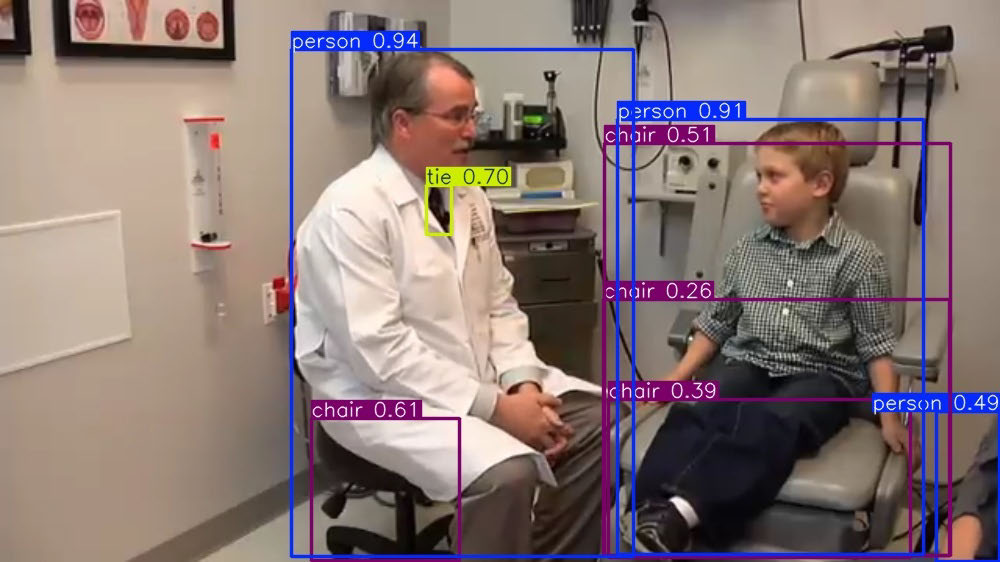
\includegraphics[width=0.9\textwidth]{images/fig-010.jpg} \\
            \vspace{0.2cm}
            \scriptsize{Comparative analysis: Standard NMS (left) vs. Specialized Spatial Fine-tuning (right).}
        \end{column}
    \end{columns}
\end{frame}

% 6. Methodology II
\begin{frame}{Methodology II: Tracking the Biological Entity}
    \begin{columns}
        \begin{column}{0.6\textwidth}
            \textbf{The Neuro-Symbolic Pipeline:}
            \begin{itemize}
                \item \textbf{Detection:} YOLOv11 extracts pixel-level precision masks.
                \item \textbf{Persistence:} How do we avoid double-counting if someone is occluded?
            \end{itemize}
            \textbf{Kalman Filter Prediction-Correction Loop:}
            \begin{block}{Prediction (Kinematics)}
                $\hat{x}_k^- = F\hat{x}_{k-1} + Bu_k$ \quad ; \quad $P_k^- = FP_{k-1}F^T + Q$
            \end{block}
            \begin{block}{Correction (Update)}
                $\hat{x}_k = \hat{x}_k^- + K_k(z_k - H\hat{x}_k^-)$
            \end{block}
            This mathematical engine ensures IDs remain persistent across complex spatial overlaps.
        \end{column}
        \begin{column}{0.4\textwidth}
            \centering
            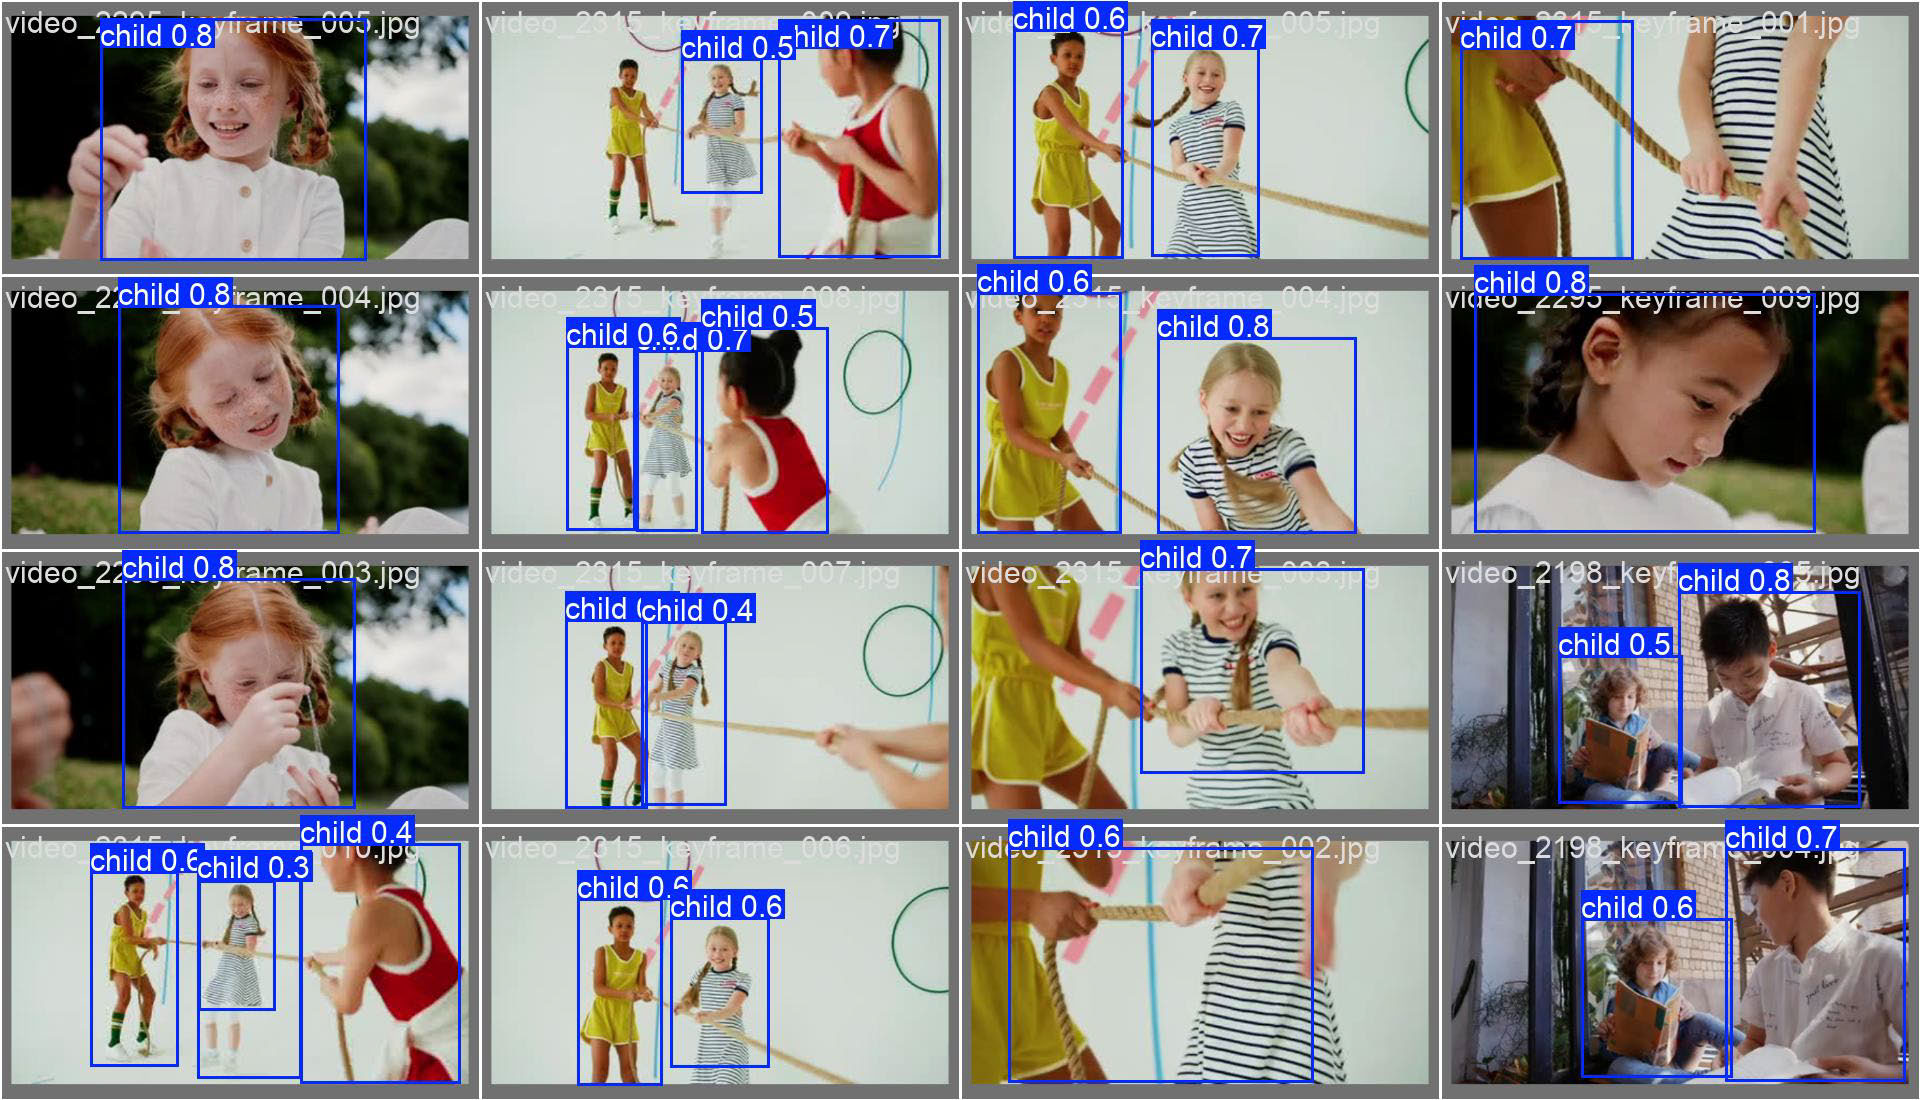
\includegraphics[width=0.9\textwidth]{images/fig-008.jpg} \\
            \vspace{0.2cm}
            \scriptsize{Training baseline: Diverse postures from the Child Detection Dataset.}
        \end{column}
    \end{columns}
\end{frame}
